% % % % % % % % % % % % % % % % % % % % % % % % % % % % % % % % % % % % % % % % % % % %
%                                                                                     %
% Short Sectioned Assignment LaTeX Template Version 1.0 (5/5/12)                      %
% This template has been downloaded from: http://www.LaTeXTemplates.com               %
%                                                                                     %
% Original author:  Frits Wenneker (http://www.howtotex.com)                          %
%                                                                                     %
% Modified by: Fco Javier Sueza Rodríguez (fcosueza@disroot.org)                      %
%                                                                                     %
% Changes:                                                                            %
%	    - Custom Chapters, Sections and Subsections (titlesec package)                %
%           - Document type scrbook (oneside)                                         %
%           - Use babel-lang-spanish package and marvosym                             %
%           - Use hyperref, enumitem, tcolorbox and glossaries packages               %
%           - Use Time New Roman (mathptmx), Helvetic and Courier fonts               %
%                                                                                     %
% License: CC BY-NC-SA 3.0 (http://creativecommons.org/licenses/by-nc-sa/3.0/)        %
%                                                                                     %
% % % % % % % % % % % % % % % % % % % % % % % % % % % % % % % % % % % % % % % % % % % %

%-----------------------------------------------%
%	              Packages                  %
%-----------------------------------------------%

\documentclass[paper=a4, fontsize=11pt, oneside]{scrbook}

% ---- Text Input/Output ----- %

\usepackage[T1]{fontenc}
\usepackage[utf8]{inputenc}
\usepackage{mathptmx}
\usepackage[scaled=.92]{helvet}
\usepackage{courier}
\usepackage[indent=12pt]{parskip}

\usepackage{geometry}
\geometry{verbose,tmargin=3cm,bmargin=3cm,lmargin=2.6cm,rmargin=2.6cm}

% ---- Language ----- %

\usepackage[spanish]{babel}
\usepackage{marvosym}

% ---- Another packages ---- %

\usepackage{amsmath,amsfonts,amsthm}
\usepackage{graphics,graphicx}
\usepackage{titlesec}
\usepackage{fancyhdr}
\usepackage{tcolorbox}
\usepackage{hyperref}
\usepackage{enumitem}
\usepackage[automake]{glossaries}

%--------------------------------------------------------------------%
%                      Customizing Document                          %
%--------------------------------------------------------------------%


% ----------- Custom Chapters, Sections and Subsections -------------- %

\titleformat{\chapter}[display]
			{\bfseries\Huge}
			{Tema \ \thechapter} {0.5ex}
			{\vspace{1ex}\centering}

\titleformat{\section}[hang]
			{\bfseries\Large}
			{\thesection}{0.5em}{}

\titleformat{\subsection}[hang]
			{\bfseries\large}
			{\thesubsection}{0.5em}{}

\titleformat{\subsubsection}[hang]
			{\bfseries\large}
			{\thesubsubsection}{0.5em}{}

\hypersetup{
    colorlinks=true,
    linkcolor=black,
    urlcolor=magenta
}

% ------------------- Custom heaaders and footers ------------------- %

\pagestyle{fancyplain}

\fancyhead[]{}
\fancyfoot[L]{}
\fancyfoot[C]{}
\fancyfoot[R]{\thepage}

\renewcommand{\headrulewidth}{0pt} % Remove header underlines
\renewcommand{\footrulewidth}{0pt} % Remove footer underlines

\setlength{\headheight}{13.6pt} % Customize the height of the header

% --------- Numbering equations, figures and tables ----------------- %

\numberwithin{equation}{section} % Number equations within sections
\numberwithin{figure}{section} % Number figures within sections
\numberwithin{table}{section} % Number tables within sections

% ------------------------ New Commands ----------------------------- %

\newcommand{\horrule}[1]{\rule{\linewidth}{#1}} % Create horizontal rule command


%----------------------------------------------------------------------------------------
%	TÍTULO Y DATOS DEL ALUMNO
%----------------------------------------------------------------------------------------

\title{
\vspace{10ex}
\normalfont \normalsize
\huge \textbf{Tarea 3: Sesiones y Autenticación en PHP}
}
\author{Francisco Javier Sueza Rodríguez}
\date{\normalsize\today}

%----------------------------------------------------------------------------------------
%                                     DOCUMENTO
%----------------------------------------------------------------------------------------
\begin{document}

\maketitle

\thispagestyle{empty}

\vspace{70ex}

\begin{center}
    \begin{tabular}{l l}
        \textbf{Centro}: & IES Aguadulce \\
        \textbf{Ciclo Formativo}: & Desarrollo Aplicaciones Web (Distancia)\\
        \textbf{Asignatura}: & Desarrollo Web en Entorno Servidor\\
        \textbf{Tema}: & Tema 3 -  Sesiones y Autenticación en PHP.\\
    \end{tabular}
\end{center}

\newpage

\section*{Buscando Las Cookies}
En ese ejercicio sea ha accedido a una aplicación web, que en este caso ha sido \href{https://github.com/}{GitHub}. Como se indica en el enunciado se ha accedido en modo privado y sin iniciar sesión. Una vez hemos accedido a la página, se ha comprobado las cookies que almacena la aplicación en nuestro navegador.

Cabe esperar, que se almacene algunas cookies del siguiente tipo:

\begin{itemize}
    \item \textbf{Cookies de Sesión}: aunque no estamos loggeados en la página, es de esperar que la aplicación almacene algunas cookies de sesión, para mantener información sobre nuestra navegación por la página web, dentro de formularios, etc. Además, dentro de este tipo de cookies deberá haber alguna que especifique si estamos loggeados o no en la aplicación.

    \item \textbf{Cookies Tema de Colores}: si la aplicación, como es en este caso, adapta su tema de colores al de nuestro navegador, también es de esperar que almacene alguna cookie con esta información, de forma que pueda cargar el tema adecuado por defecto cuando accedamos a la aplicación.

    \item \textbf{Cookies con Información del Cliente}: también se pueden almacenar información sobre el cliente, como por ejemplo la zona horario donde se ubica, si se muestra algún tipo de reloj o datos que incluyan información con tiempo, como por ejemplo puede ser la información asociada a los commits, etc.
\end{itemize}

En la siguiente imagen se muestran las cookies almacenadas por Github en el navegador firefox.

    \begin{figure}[H]
    \centering
    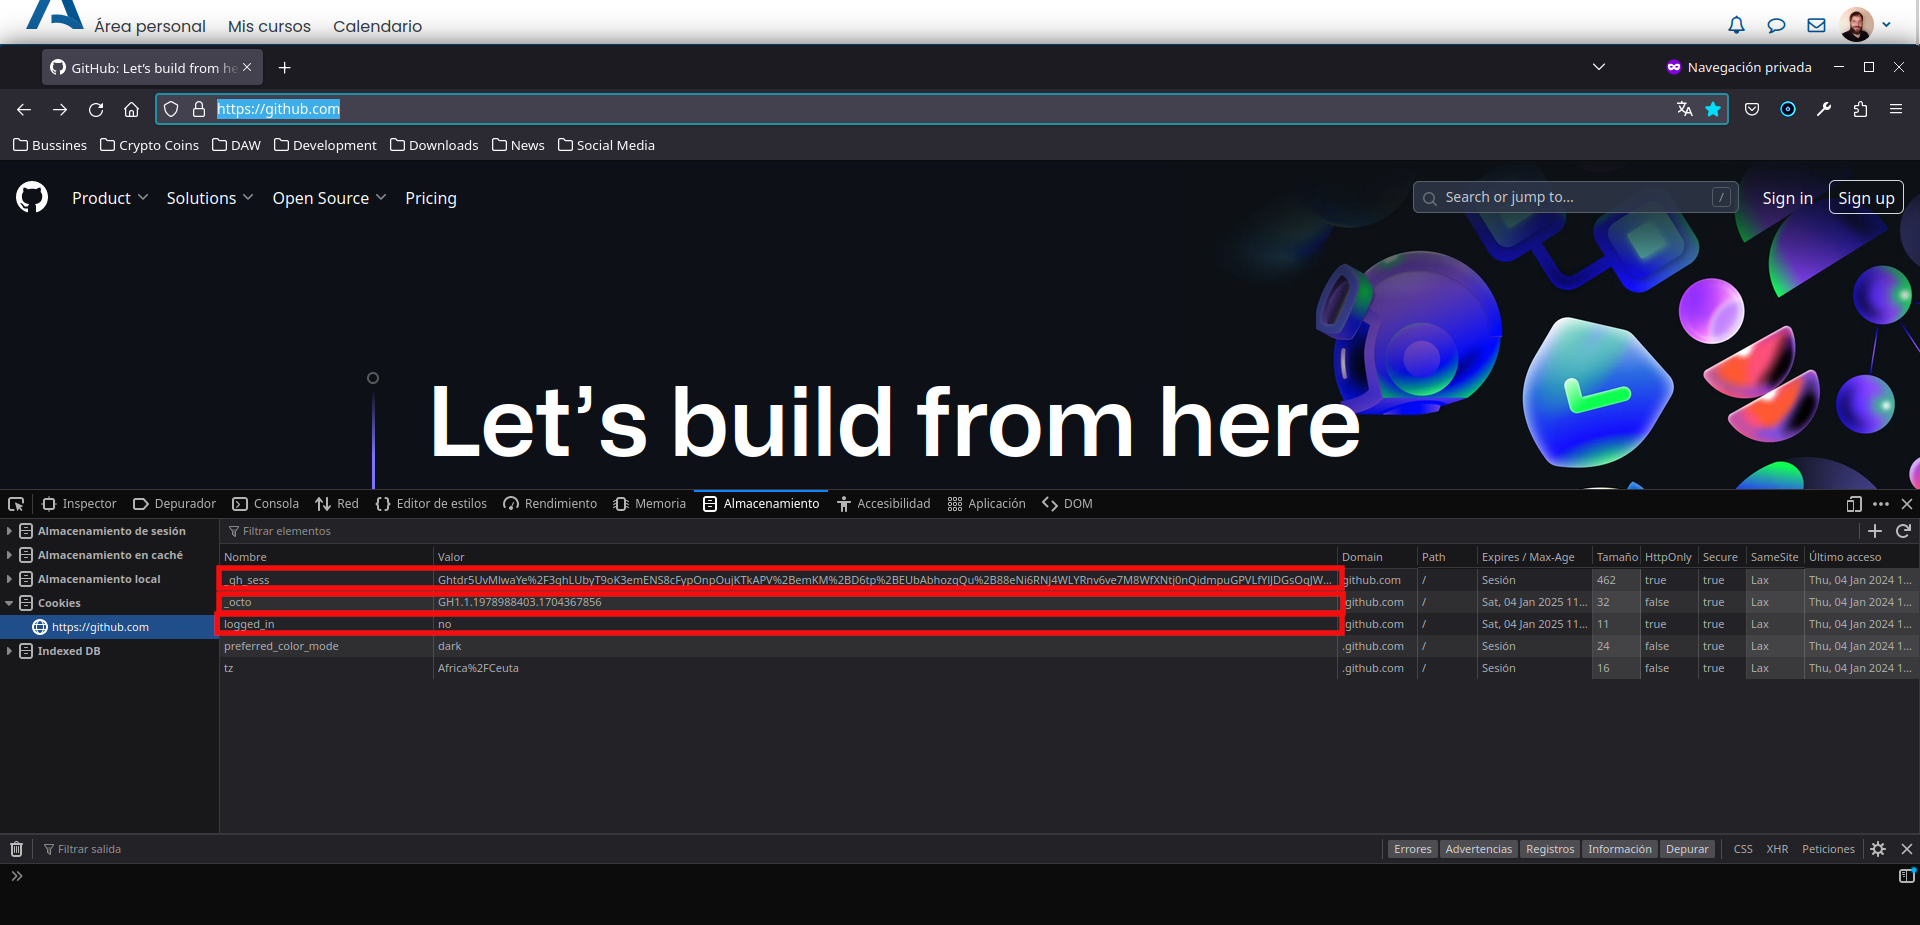
\includegraphics[scale=0.30]{cookies-github.png}
    \caption{Cookies almacenadas por Github}
\end{figure}

En la figura anterior se han remarcado la cookies de sesión que almacena Github, si haber realizado logging. Estas cookies son: \textbf{\_gh\_sess}, \textbf{\_octo} y \textbf{logged\_in}.

Aunque algunas son identificables claramente como cookies de sesión hay alguna otra, como \textbf{\_octo} en las que hemos tenido que consultar la documentación de Github sobre las cookies que emplea la aplicación, que podemos encontrar en la web: \url{https://github.com/privacy/cookies}.
% Bibliography

%\newpage
%\bibliography{citas}
%\bibliographystyle{unsrt}

\end{document}